\chapter{Synthèse totale~: stratégie et voies classiques}\label{ch:b3:total-synthesis}

L'anticancéreux paclitaxel fut d'abord isolé de l'écorce de l'if du
Pacifique, un arbre à croissance lente~; écorcer l'arbre le tuait, et
l'approvisionnement restait très loin des besoins des patients. Les
chimistes répondirent de deux façons~: des \omterm{def:b3:total-synthesis:total}{synthèses totales}, qui
montrèrent que la molécule pouvait être construite à partir de matières
premières simples mais étaient bien trop longues pour la production, et une
\omterm{def:b3:total-synthesis:total}{hémisynthèse} à partir d'un composé apparenté extrait des aiguilles d'un if
commun, ressource renouvelable. Ce chapitre explique comment juger et
concevoir de telles voies~: comment les rendements se multiplient, pourquoi
la convergence paie, ce que coûtent les groupes protecteurs, quelles
liaisons former en premier, et trois synthèses historiques lues avec ces
outils.

\begin{recall}
Le volume de deuxième année a traité de l'analyse rétrosynthétique
(molécule cible, déconnexion, synthon, équivalent synthétique,
interconversion de groupes fonctionnels), des groupes protecteurs
orthogonaux, de l'aldolisation, de l'annélation de Robinson, de la réaction
de Wittig et de la chimie des iminiums~; le volume de première année, des
groupes protecteurs et des rendements. Le
\cref{ch:b3:asymmetric-synthesis}, le \cref{ch:b3:pericyclic} et le
\cref{ch:b3:homogeneous-catalysis} ont fourni les étapes clés modernes.
\end{recall}

\begin{omfigure}
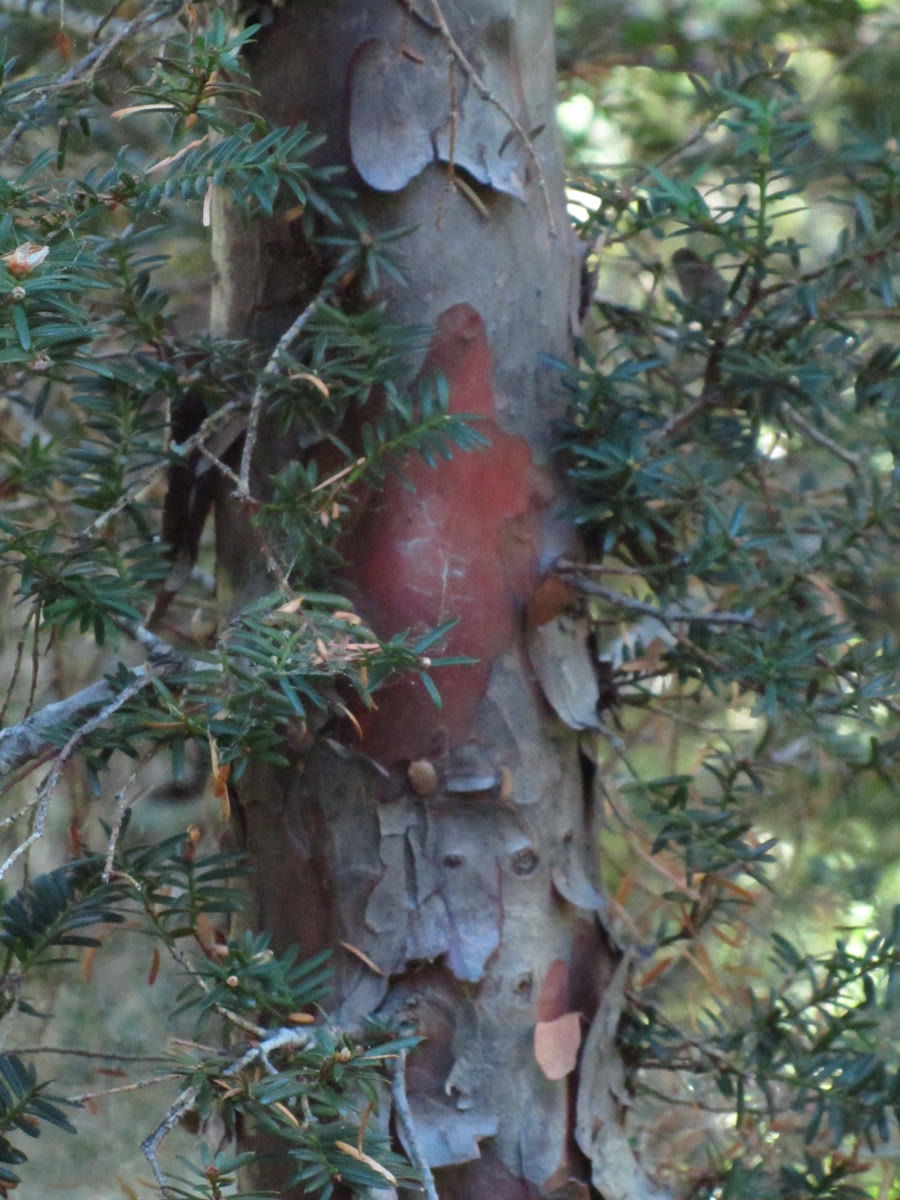
\includegraphics[width=0.32\linewidth]{images/book4/pacific-yew.jpg}

{\small Écorce et aiguilles d'un if du Pacifique, première source de
paclitaxel. Photographie~: JOE BLOWE, CC BY-SA 2.0.}
\end{omfigure}

\section{Mesurer une synthèse}

\begin{definition}[Synthèse totale]\label{def:b3:total-synthesis:total}
Une \emph{synthèse totale}\index{synthese totale@synthèse totale} prépare une molécule complexe,
souvent un produit naturel, à partir de composés commerciaux simples. Une
\emph{synthèse formelle}\index{synthese formelle@synthèse formelle} prépare un intermédiaire d'une
synthèse totale antérieure, ce qui achève la voie sur le papier. Une
\emph{hémisynthèse}\index{hemisynthese@hémisynthèse} part d'un composé naturel déjà proche de
la cible.
\end{definition}

\begin{definition}[Architecture d'une voie]\label{def:b3:total-synthesis:architecture}
Dans une \emph{synthèse linéaire}\index{synthese lineaire@synthèse linéaire}, chaque étape agit sur
le produit de la précédente~; dans une \emph{synthèse convergente}\index{synthese convergente@synthèse convergente},
des fragments distincts sont préparés en parallèle et assemblés tard. La
\emph{plus longue séquence linéaire}\index{plus longue sequence lineaire@plus longue séquence linéaire} (LLS) est le plus grand
nombre d'étapes séparant une matière première de la cible. Le
\emph{rendement global}\index{rendement global} est la quantité de cible
obtenue divisée par la quantité de la matière première limitante.
\end{definition}

\begin{proposition}[Rendement global]\label{prop:b3:total-synthesis:overall-yield}
Pour une suite d'étapes de rendements $y_1, \dots, y_n$, le \omterm{def:b3:total-synthesis:architecture}{rendement global} vaut $Y = \prod_i y_i$.
\end{proposition}

\begin{proof}
Chaque étape convertit la quantité qu'elle reçoit en $y_i$ fois autant de produit~; la
quantité qui atteint la cible est la quantité de départ multipliée
successivement par chaque facteur.
\end{proof}

\begin{proposition}[Convergence]\label{prop:b3:total-synthesis:convergent}
Une voie de $n = 2m + 1$ étapes de même rendement $y$, construite en deux branches de $m$ étapes reliées par
une étape de couplage, a un \omterm{def:b3:total-synthesis:architecture}{rendement global} de $y^{m+1}$ le long de sa \omterm{def:b3:total-synthesis:architecture}{plus longue séquence linéaire},
contre $y^{2m+1}$ pour la voie linéaire formée des mêmes étapes.
\end{proposition}

\begin{proof}
Chaque branche est préparée séparément, à partir d'autant de matière
première que nécessaire~: la matière de chaque branche traverse $m$ étapes puis le couplage, $m + 1$
facteurs $y$. Dans la voie linéaire, la matière les traverse toutes, $2m + 1$. Pour $m = 10$
et $y = 0.90$~: 31\,\% contre 11\,\%.
\end{proof}

\begin{omfigure}
\begin{tikzpicture}
\begin{axis}[width=0.7\linewidth, height=5.8cm, xmin=0, xmax=30, ymin=0, ymax=1.02,
  axis lines=left, xlabel={nombre d'étapes $n$}, ylabel={rendement global},
  tick label style={font=\scriptsize}, label style={font=\small},
  legend style={font=\scriptsize, draw=none, at={(1.03,0.5)}, anchor=west}, legend cell align=left]
\addplot[color=omDef, thick] table[x=n, y=y95] {figdata/out/bachelor-3-overall-yield.dat};
\addlegendentry{95\,\% par étape}
\addplot[color=omMeth, thick] table[x=n, y=y90] {figdata/out/bachelor-3-overall-yield.dat};
\addlegendentry{90\,\%}
\addplot[color=omThm, thick] table[x=n, y=y80] {figdata/out/bachelor-3-overall-yield.dat};
\addlegendentry{80\,\%}
\addplot[color=omMeth, thick, dashed, mark=*, mark size=1pt] table[x=n, y=y90] {figdata/out/bachelor-3-overall-yield-b.dat};
\addlegendentry{90\,\%, convergente}
\end{axis}
\end{tikzpicture}

{\small \omterm{def:b3:total-synthesis:architecture}{Rendement global} en fonction du nombre d'étapes pour trois
rendements par étape (traits pleins~: voies linéaires), et pour des voies
convergentes à 90\,\% par étape (deux branches égales assemblées lors d'une
dernière étape~; tirets). Vingt étapes à 90\,\% laissent 12\,\%~; les mêmes
étapes organisées de façon convergente en laissent environ trois fois
plus.}
\end{omfigure}

\begin{omfigure}
\begin{tikzpicture}[font=\scriptsize, >=Stealth, node distance=0.9cm,
  st/.style={circle, draw, fill=omDef!15, minimum size=4mm, inner sep=0pt}]
  \foreach \i in {0,...,6} { \node[st] (l\i) at (\i*0.9,1.6) {}; }
  \foreach \i in {0,...,5} { \pgfmathtruncatemacro\j{\i+1} \draw[->] (l\i) -- (l\j); }
  \node[anchor=west] at (6.0,1.6) {linéaire~: 6 étapes, LLS 6};
  \foreach \i in {0,...,2} { \node[st] (a\i) at (\i*0.9,0.6) {}; \node[st] (b\i) at (\i*0.9,-0.6) {}; }
  \draw[->] (a0) -- (a1); \draw[->] (a1) -- (a2); \draw[->] (b0) -- (b1); \draw[->] (b1) -- (b2);
  \node[st, fill=omThm!25] (t) at (3.0,0) {};
  \draw[->] (a2) -- (t); \draw[->] (b2) -- (t);
  \node[anchor=west] at (3.4,0) {convergente~: 5 étapes, LLS 3};
\end{tikzpicture}

{\small Arbres de voies~: chaque cercle est un composé, chaque flèche une
étape. Une voie linéaire fait passer toute sa matière par chaque étape~;
une voie convergente prépare deux fragments côte à côte et les couple, si
bien que sa \omterm{def:b3:total-synthesis:architecture}{plus longue séquence linéaire} est plus courte.}
\end{omfigure}

\begin{definition}[Économies et idéalité]\label{def:b3:total-synthesis:economy}
L'\emph{économie d'étapes}\index{economie d'etapes@économie d'étapes} est l'objectif d'atteindre une
cible en aussi peu d'étapes que possible~; l'\emph{économie de groupes protecteurs}\index{economie de groupes protecteurs@économie de groupes protecteurs},
celui d'utiliser aussi peu d'étapes de protection et de déprotection que
possible. L'\emph{idéalité}\index{idealite@idéalité} d'une voie est la fraction de ses étapes
qui construisent le squelette ou réalisent un changement nécessaire de
degré d'oxydation~:
$(\text{étapes de construction} + \text{étapes redox stratégiques})/(\text{nombre total d'étapes})$.
\end{definition}

\begin{proposition}[Idéalité d'une voie]\label{prop:b3:total-synthesis:ideality}
Une voie monotope qui ne forme que des liaisons du squelette a une \omterm{def:b3:total-synthesis:economy}{idéalité}
de 100\,\%~; chaque étape de protection, de déprotection, d'interconversion
de groupes fonctionnels ou d'oxydoréduction non stratégique la diminue.
\end{proposition}

\begin{proof}
Directement d'après la définition~: de telles étapes s'ajoutent au
dénominateur sans s'ajouter au numérateur.
\end{proof}

\section{Les groupes protecteurs et leur économie}

Chaque groupe protecteur coûte au moins deux étapes, les réactifs pour le
poser et l'ôter, et la matière perdue lors des deux. Une voie de huit
étapes à 90\,\% conserve 43\,\% de sa matière~; ajouter deux protections et
deux déprotections à 95\,\% chacune la ramène à 35\,\%. On choisit des
groupes protecteurs orthogonaux, de sorte que chacun puisse être retiré
sans toucher aux autres~; mieux encore, on ordonne les étapes de sorte que
le groupe réactif soit absent, ou pas encore révélé, quand il gênerait~: les
synthèses sans groupe protecteur sont un objectif, non une curiosité.

\begin{method}[Lire une synthèse totale]\label{met:b3:total-synthesis:analyse}
\begin{enumerate}
  \item Repérer les cycles, les stéréocentres et les groupes sensibles de
        la cible.
  \item Trouver les déconnexions clés et les réactions qui les réalisent
        dans le sens direct (\omterm{def:b3:total-synthesis:strategic-bond}{liaisons stratégiques}).
  \item Compter les étapes et trouver la \omterm{def:b3:total-synthesis:architecture}{plus longue séquence linéaire}~;
        noter la convergence.
  \item Noter comment chaque stéréocentre est créé (contrôle par le
        substrat, auxiliaire, catalyseur, \omterm{def:b3:asymmetric-synthesis:chiral-pool}{réservoir chiral}).
  \item Lister les groupes protecteurs et les autres étapes non idéales~;
        calculer le \omterm{def:b3:total-synthesis:architecture}{rendement global} et l'\omterm{def:b3:total-synthesis:economy}{idéalité}.
\end{enumerate}
\end{method}

\begin{method}[Compter les étapes]\label{met:b3:total-synthesis:count}
\begin{enumerate}
  \item Une étape est une opération qui se termine par un produit isolé
        (ou au moins traité)~; une séquence monotope sans isolement compte
        pour une étape.
  \item Compter toutes les étapes pour le total~; pour la LLS, suivre le
        plus long chemin d'un composé commercial à la cible.
  \item Multiplier les rendements le long de la LLS pour obtenir le
        \omterm{def:b3:total-synthesis:architecture}{rendement global}.
\end{enumerate}
\end{method}

\section{Liaisons stratégiques et étapes clés de formation de cycles}

\begin{definition}[Liaison stratégique]\label{def:b3:total-synthesis:strategic-bond}
Une \emph{liaison stratégique} d'une cible\index{liaison strategique@liaison stratégique} est une liaison dont
la déconnexion simplifie le plus la cible, en général en scindant un
système de cycles ou en supprimant plusieurs stéréocentres à la fois, et
qu'une réaction fiable sait former.
\end{definition}

Les réactions de formation de cycles qui créent deux liaisons ou plusieurs
stéréocentres à la fois sont les chevaux de bataille~: la réaction de
Diels--Alder (deux liaisons C--C, jusqu'à quatre stéréocentres, de façon
stéréospécifique, \cref{ch:b3:pericyclic}), l'annélation de Robinson (un
cycle à six chaînons sur une cétone), la \omterm{def:b3:homogeneous-catalysis:metathesis}{métathèse cyclisante}
(\cref{ch:b3:homogeneous-catalysis}) pour les cycles moyens et grands, et
les cascades.

\begin{definition}[Réaction en cascade]\label{def:b3:total-synthesis:cascade}
Une \emph{réaction en cascade}\index{reaction en cascade@réaction en cascade} est une suite de
transformations dans laquelle chaque étape crée la fonctionnalité
nécessaire à la suivante, sans isolement d'intermédiaires ni ajout de
réactifs.
\end{definition}

\begin{definition}[Synthèse biomimétique]\label{def:b3:total-synthesis:biomimetic}
Une \emph{synthèse biomimétique}\index{synthese biomimetique@synthèse biomimétique} imite la voie
par laquelle on pense qu'un produit naturel est fabriqué dans l'organisme.
\end{definition}

La cyclisation de l'oxyde de squalène en lanostérol dans les cellules,
quatre cycles et sept stéréocentres en une seule cascade enzymatique, a
inspiré les cyclisations de polyènes de William Johnson, dans lesquelles un
cation créé à une extrémité d'un polyène soigneusement conçu ferme cycle
après cycle par des états de transition de type chaise, en fixant les
jonctions de cycles \textit{trans} des stéroïdes.

\section{Voies historiques}

\begin{definition}[Réaction de Mannich]\label{def:b3:total-synthesis:mannich}
La \emph{réaction de Mannich}\index{reaction de Mannich@réaction de Mannich} est l'addition d'un
énol ou d'un énolate sur un ion iminium, formé in situ à partir d'un
aldéhyde et d'une amine primaire ou secondaire, qui donne un composé carbonylé $\beta$-aminé.
\end{definition}

En 1917, Robert Robinson prépara la tropinone, le cœur bicyclique de
l'atropine et de la cocaïne, en un seul pot à partir de trois composants
simples dans l'eau, en imaginant que la plante pourrait la construire de la
même façon~:
$\ce{C4H6O2 + CH3NH2 + C5H6O5 -> C8H13NO + 2CO2 + 2H2O}$ (le succinaldéhyde, la méthylamine et
l'acide acétonedicarboxylique donnent la tropinone).

\begin{omfigure}
\begin{tikzpicture}[font=\small, >=Stealth]
  \node[align=center] at (-0.5,0) {$\ce{OHC-CH2CH2-CHO}$\\ $+\ \ce{CH3NH2}$\\ $+\ \ce{HO2C-CH2-CO-CH2-CO2H}$};
  \draw[->, thick] (3.0,0) -- (4.7,0) node[midway, above, font=\scriptsize] {eau tamponnée} node[midway, below, font=\scriptsize] {$-\ce{2CO2}$, $-\ce{2H2O}$};
  \begin{scope}[xshift=6.1cm, yshift=-0.2cm]
    \coordinate (c1) at (-1,0.3); \coordinate (c2) at (-0.8,-0.5); \coordinate (c3) at (0,-0.9);
    \coordinate (c4) at (0.8,-0.5); \coordinate (c5) at (1,0.3); \coordinate (c6) at (0.45,1.15);
    \coordinate (c7) at (-0.45,1.15); \coordinate (n) at (0,0.45);
    \draw[thick] (c1) -- (c2) -- (c3) -- (c4) -- (c5) -- (c6);
    \draw[thick] (c7) -- (c1);
    \draw[thick] (c6) -- (0.12,1.15); \draw[thick] (-0.12,1.15) -- (c7);
    \draw[thick] (c1) -- (n) -- (c5);
    \draw[thick] (n) -- (0,1.6) node[above, inner sep=1pt] {$\ce{CH3}$};
    \draw[thick, double, double distance=1.5pt] (c3) -- (0,-1.55) node[below, inner sep=1pt] {O};
    \node[fill=white, inner sep=0.5pt] at (n) {N};
    \node[font=\scriptsize, anchor=west] at (1.2,0.3) {tropinone};
  \end{scope}
\end{tikzpicture}

{\small La synthèse de la tropinone de Robinson. Deux \omterm{def:b3:total-synthesis:mannich}{réactions de Mannich},
la première intermoléculaire et la seconde qui ferme le cycle, réunissent
les trois composants~; les deux groupes acide carboxylique qui rendaient
énolisables les groupes $\ce{CH2}$ centraux partent ensuite sous forme de dioxyde de
carbone. Dans le produit bicyclique, le pont N-méthyle enjambe le cycle à
sept chaînons.}
\end{omfigure}

\begin{proposition}[La tropinone en un seul pot]\label{prop:b3:total-synthesis:tropinone}
La synthèse monotope de la tropinone se compose de deux \omterm{def:b3:total-synthesis:mannich}{réactions de
Mannich} suivies de deux décarboxylations.
\end{proposition}

\begin{proof}[Justification]
La méthylamine et un groupe aldéhyde du succinaldéhyde donnent un ion
iminium~; un énol de l'acide acétonedicarboxylique s'y additionne (première
\omterm{def:b3:total-synthesis:mannich}{réaction de Mannich}). L'amine secondaire formée se condense avec le second
groupe aldéhyde en un ion iminium cyclique, que l'énol situé de l'autre
côté de la cétone attaque (seconde \omterm{def:b3:total-synthesis:mannich}{réaction de Mannich}), ce qui ferme le
bicycle. Les deux groupes $\beta$-céto-acide perdent ensuite $\ce{CO2}$, comme le font les $\beta$-céto-acides
par léger chauffage.
\end{proof}

La synthèse de la prostaglandine $\mathrm F_{2\alpha}$ par Elias Corey (1969) a rendu l'analyse
rétrosynthétique explicite. Une bicyclo[2.2.1]hepténone construite par une
réaction de Diels--Alder porte la configuration relative des substituants
du cyclopentane~; une \omterm{def:b3:radicals-carbenes:baeyer}{oxydation de Baeyer--Villiger}
(\cref{ch:b3:radicals-carbenes}) et une iodolactonisation la transforment
en lactone de Corey, sur laquelle les deux chaînes latérales sont fixées
par des oléfinations. Cette lactone a servi depuis pour de nombreux
médicaments prostaglandines.

\begin{omfigure}
\begin{tikzpicture}[font=\small,
  box/.style={draw, rounded corners, align=center, fill=omDef!8, inner sep=4pt}]
  \node[box] (t) at (0,0) {prostaglandine\\ $\mathrm F_{2\alpha}$};
  \node[box] (l) at (4.4,0) {lactone de Corey\\ (quatre\\ stéréocentres)};
  \node[box] (b) at (9.2,0) {bicyclo[2.2.1]-\\ hepténone};
  \node[box] (d) at (9.2,-2.4) {cyclopentadiène\\ substitué $+$\\ équivalent de cétène};
  \draw[omretro] (t) -- (l) node[midway, above=3pt, font=\scriptsize] {oléfinations};
  \draw[omretro] (l) -- (b) node[midway, above=3pt, font=\scriptsize, align=center] {\tiny iodolactonisation,\\ \tiny Baeyer--Villiger};
  \draw[omretro] (b) -- (d) node[midway, right, font=\scriptsize] {Diels--Alder};
\end{tikzpicture}

{\small La rétrosynthèse de la prostaglandine $\mathrm F_{2\alpha}$ par Corey, dans les grandes lignes (flèches doubles~: «~est
préparé à partir de~»). Les deux chaînes latérales sont déconnectées en
premier~; le cyclopentane et ses quatre stéréocentres proviennent d'une
lactone, la lactone d'une cétone bicyclique, et la cétone d'une réaction de
Diels--Alder qui fixe leur configuration relative.}
\end{omfigure}

L'oseltamivir, le médicament contre la grippe, est fabriqué industriellement
à partir de l'acide shikimique, un composé du \omterm{def:b3:asymmetric-synthesis:chiral-pool}{réservoir chiral} extrait de
l'anis étoilé puis produit par fermentation~: son cycle à six chaînons et
ses stéréocentres sont déjà en place. La voie transforme le diol du cycle
en époxyde, l'ouvre par l'azoture, ferme une aziridine et l'ouvre de
nouveau par l'azoture, ce qui place les deux atomes d'azote en
\textit{trans}~; une acétylation et une réduction achèvent le travail. Comme l'azoture
de sodium et les azotures organiques sont toxiques et potentiellement
explosifs à grande échelle, des voies sans azoture furent développées par
la suite.

\begin{omfigure}
\begin{tikzpicture}[font=\scriptsize, >=Stealth,
  box/.style={draw, rounded corners, align=center, fill=omMeth!8, inner sep=3pt}]
  \node[box] (a) at (0,0) {acide ($-$)-shikimique\\ (réservoir chiral)};
  \node[box] (b) at (3.1,0) {ester, cétal,\\ mésylate};
  \node[box] (c) at (6.0,0) {époxyde};
  \node[box] (d) at (8.6,0) {azidoalcool};
  \node[box] (e) at (8.6,-1.5) {aziridine};
  \node[box] (f) at (5.4,-1.5) {précurseur de la\\ \textit{trans}-diamine\\ (azoture)};
  \node[box] (g) at (1.6,-1.5) {phosphate\\ d'oseltamivir};
  \draw[->] (a) -- (b); \draw[->] (b) -- (c); \draw[->] (c) -- (d) node[midway, above] {$\ce{N3-}$};
  \draw[->] (d) -- (e); \draw[->] (e) -- (f) node[midway, above] {$\ce{N3-}$};
  \draw[->] (f) -- (g) node[midway, below, align=center] {acétylation,\\ réduction};
\end{tikzpicture}

{\small L'oseltamivir à partir de l'acide shikimique, étapes clés
seulement~: le cycle naturel et ses stéréocentres sont conservés, et deux
atomes d'azote sont introduits en \textit{trans} l'un de l'autre par les ouvertures
successives d'un époxyde et d'une aziridine par l'azoture.}
\end{omfigure}

\section{De la découverte au procédé}

Une voie qui fournit des milligrammes pour les essais biologiques est
rarement celle qu'on utilise pour des tonnes. Les chimistes de procédé
explorent les voies selon leur coût, leur sécurité et leur robustesse~: ils
remplacent la chromatographie par la cristallisation, éliminent les
réactifs dangereux et les températures cryogéniques, raccourcissent la
séquence, vérifient par calorimétrie la sécurité thermique de chaque étape
et fixent des spécifications pour les impuretés. Ces choix rejoignent les
mesures du \cref{ch:b3:green-industrial}.

\begin{inthelab}[D'un gramme à un kilogramme]
Une étape menée sur un gramme dans un ballon à fond rond est répétée sur
dix grammes dans un réacteur à double enveloppe muni d'une agitation
mécanique et d'une sonde de température plongeant dans le liquide, en
ajoutant le réactif le plus réactif à vitesse contrôlée tout en surveillant la
température interne~: la chaleur dégagée croît avec le volume, mais la
surface qui l'évacue ne croît qu'avec le carré de la taille. Ce n'est que
lorsque le flux de chaleur et le traitement (séparations de phases,
filtrations, séchage) se comportent bien que l'étape est menée sur un
kilogramme.
\end{inthelab}

\begin{safety}{\ghs[0.62cm]{GHS06}\ghs[0.62cm]{GHS08}\ghs[0.62cm]{GHS09}}
% ledger: ghs4:NaN3
Azoture de sodium~: mortel en cas d'ingestion, très toxique pour les
organismes aquatiques~; avec les acides, il libère de l'acide
azothydrique, gaz toxique et explosif, et avec les métaux lourds (cuivre et
plomb des canalisations) il forme des azotures explosifs. Les déchets sont
détruits chimiquement, jamais jetés à l'évier.
\end{safety}

\begin{history}[Robinson, Woodward, Corey]
Robert Robinson reçut le prix Nobel de chimie 1947 pour ses travaux sur les
alcaloïdes et d'autres produits végétaux~; sa synthèse de la tropinone de
1917 est encore citée pour son économie. Les synthèses de la quinine, du
cholestérol, de la chlorophylle et, avec Albert Eschenmoser, de la vitamine $\mathrm B_{12}$ par Robert Woodward firent de la \omterm{def:b3:total-synthesis:total}{synthèse totale} un art
(prix 1965). Elias Corey formalisa l'analyse rétrosynthétique et reçut le
prix 1990 pour la théorie et la méthodologie de la synthèse organique.
\end{history}

\section{Exercices}

\begin{exercise}[$\star$]\label{exo:b3:total-synthesis:1}
Calculer le \omterm{def:b3:total-synthesis:architecture}{rendement global} de voies linéaires de 10 et de 20 étapes à
90\,\% et à 80\,\% par étape.
\end{exercise}

\begin{exercise}[$\star$]\label{exo:b3:total-synthesis:2}
Une voie prépare le fragment A en cinq étapes et le fragment B en trois,
les couple, puis exige quatre étapes de plus jusqu'à la cible. Donner le
nombre total d'étapes et la \omterm{def:b3:total-synthesis:architecture}{plus longue séquence linéaire}.
\end{exercise}

\begin{exercise}[$\star$]\label{exo:b3:total-synthesis:3}
Donner le produit de la \omterm{def:b3:total-synthesis:mannich}{réaction de Mannich} de l'acétone, du méthanal et
de la diméthylamine.
\end{exercise}

\begin{exercise}[$\star$]\label{exo:b3:total-synthesis:4}
Donner une déconnexion de Diels--Alder du 4-acétylcyclohexène, et la
réaction dans le sens direct.
\end{exercise}

\begin{exercise}[$\star\star$]\label{exo:b3:total-synthesis:5}
Une voie linéaire de 21 étapes fonctionne à 90\,\% par étape. Calculer son
\omterm{def:b3:total-synthesis:architecture}{rendement global} et celui d'une version convergente à deux branches de 10
étapes et un couplage.
\end{exercise}

\begin{exercise}[$\star\star$]\label{exo:b3:total-synthesis:6}
La voie A compte 12 étapes, dont 7 forment des liaisons du squelette et 1
est une réduction stratégique~; la voie B compte 9 étapes, dont 7 forment
le squelette. Calculer leurs \omterm{def:b3:total-synthesis:economy}{idéalités}.
\end{exercise}

\begin{exercise}[$\star\star$]\label{exo:b3:total-synthesis:7}
Une voie de huit étapes à 90\,\% par étape exige deux groupes protecteurs,
chacun posé et retiré à 95\,\%. Calculer le \omterm{def:b3:total-synthesis:architecture}{rendement global} avec et sans
eux.
\end{exercise}

\begin{exercise}[$\star\star$]\label{exo:b3:total-synthesis:8}
Un triol possède un groupe hydroxy primaire, un secondaire et un tertiaire.
Proposer des groupes protecteurs qui permettent de révéler chacun à son
tour, et leurs conditions d'élimination.
\end{exercise}

\begin{exercise}[$\star\star$]\label{exo:b3:total-synthesis:9}
Pourquoi le paclitaxel a-t-il été produit par \omterm{def:b3:total-synthesis:total}{hémisynthèse} plutôt que par
l'une quelconque de ses \omterm{def:b3:total-synthesis:total}{synthèses totales}~?
\end{exercise}

\begin{exercise}[$\star\star\star$]\label{exo:b3:total-synthesis:10}
La 2-méthylcyclohexane-1,3-dione réagit avec la méthylvinylcétone dans une
annélation de Robinson. Identifier les étapes de Michael et d'aldolisation
et donner l'énone bicyclique formée (la cétone de Wieland--Miescher).
\end{exercise}

\begin{exercise}[$\star\star\star$]\label{exo:b3:total-synthesis:11}
Montrer que la voie convergente de la \cref{prop:b3:total-synthesis:convergent}
conserve $y^{-m}$ fois plus de matière que la voie linéaire, et évaluer ce facteur pour $m = 5$ et
$m = 15$ à 90\,\%.
\end{exercise}

\begin{exercise}[$\star\star\star$]\label{exo:b3:total-synthesis:12}
Dans une cyclisation de polyène, pourquoi les états de transition de type chaise donnent-ils des jonctions de cycles \textit{trans},
et pourquoi la géométrie (\textit{E} ou \textit{Z}) de chaque double liaison importe-t-elle~?
\end{exercise}

\section{Problème~: la tropinone en un seul pot}

\begin{problem}[{Problème du week-end --- la tropinone en un seul pot~: les
trois composants et l'équation équilibrée, les deux réactions de Mannich,
une comparaison avec une longue voie linéaire, et la stéréochimie de la
tropinone et de ses produits de réduction}]
\label{pb:b3:total-synthesis:1}
% ledger: aw:C, aw:H, aw:N, aw:O
Données du problème~: la synthèse monotope, menée dans l'eau tamponnée vers
pH 5, donne la tropinone avec 42\,\% de rendement~; une voie linéaire plus
ancienne exige 14 étapes de rendement moyen 75\,\%.

\medskip\noindent\textbf{Partie I --- Composants et équation.}
\begin{enumerate}
  \item Donner les formules du succinaldéhyde, de la méthylamine, de
        l'acide acétonedicarboxylique et de la tropinone.
  \item Écrire l'équation équilibrée.
  \item Calculer les masses molaires des réactifs et de la tropinone.
  \item Calculer l'économie d'atomes.
  \item Pourquoi utilise-t-on l'acide acétonedicarboxylique plutôt que
        l'acétone~?
  \item Pourquoi un tampon proche de la neutralité aide-t-il~?
\end{enumerate}

\medskip\noindent\textbf{Partie II --- Mécanisme.}
\begin{enumerate}[resume]
  \item Écrire la formation du premier ion iminium.
  \item Représenter la première \omterm{def:b3:total-synthesis:mannich}{réaction de Mannich}.
  \item Comment le second ion iminium se forme-t-il~?
  \item Représenter la seconde \omterm{def:b3:total-synthesis:mannich}{réaction de Mannich}, qui ferme le cycle.
  \item Pourquoi les deux groupes acide carboxylique partent-ils sous forme de $\ce{CO2}$~?
  \item Compter les liaisons C--C et C--N formées.
\end{enumerate}

\medskip\noindent\textbf{Partie III --- Un seul pot contre quatorze étapes.}
\begin{enumerate}[resume]
  \item Calculer le \omterm{def:b3:total-synthesis:architecture}{rendement global} de la voie linéaire.
  \item Calculer le rapport du rendement monotope à ce rendement.
  \item Calculer l'\omterm{def:b3:total-synthesis:economy}{idéalité} de la voie monotope.
  \item Qu'est-ce qui, outre le rendement, favorise la voie monotope~?
  \item Pourquoi dit-on que la synthèse monotope est biomimétique~?
  \item Nommer une autre classe de réactions de ce chapitre qui forme
        plusieurs liaisons à la fois.
\end{enumerate}

\medskip\noindent\textbf{Partie IV --- Stéréochimie.}
\begin{enumerate}[resume]
  \item La tropinone est-elle chirale~? Trouver son \omterm{def:b3:point-groups:operation}{élément de symétrie}.
  \item Pourquoi les deux carbones têtes de pont sont-ils néanmoins des
        stéréocentres~?
  \item La réduction de la cétone donne deux alcools, la tropine et la
        pseudotropine. Quelle relation les lie~?
  \item La tropine et la pseudotropine sont-elles chirales~?
  \item Pourquoi un hydrure approche-t-il le groupe carbonyle
        préférentiellement par une face~?
  \item Énoncer le résultat~: le rapport du rendement monotope au \omterm{def:b3:total-synthesis:architecture}{rendement
        global} de la voie linéaire.
\end{enumerate}
\end{problem}
